%%%%%%%%%%%%%%%%%%%% author.tex %%%%%%%%%%%%%%%%%%%%%%%%%%%%%%%%%%%
%
% sample root file for your "contribution" to a contributed volume
%
% Use this file as a template for your own input.
%
%%%%%%%%%%%%%%%% Springer %%%%%%%%%%%%%%%%%%%%%%%%%%%%%%%%%%


% RECOMMENDED %%%%%%%%%%%%%%%%%%%%%%%%%%%%%%%%%%%%%%%%%%%%%%%%%%%
\documentclass[graybox]{svmult}

\usepackage[utf8]{inputenc}

% choose options for [] as required from the list
% in the Reference Guide

\usepackage{type1cm}        % activate if the above 3 fonts are
                            % not available on your system
%
\usepackage{makeidx}         % allows index generation
\usepackage{graphicx}        % standard LaTeX graphics tool
                             % when including figure files
\usepackage{multicol}        % used for the two-column index
\usepackage[bottom]{footmisc}% places footnotes at page bottom


\usepackage{newtxtext}       % 
\usepackage{newtxmath}       % selects Times Roman as basic font

% see the list of further useful packages
% in the Reference Guide

\makeindex             % used for the subject index
                       % please use the style svind.ist with
                       % your makeindex program

%%%%%%%%%%%%%%%%%%%%%%%%%%%%%%%%%%%%%%%%%%%%%%%%%%%%%%%%%%%%%%%%%%%%%%%%%%%%%%%%%%%%%%%%%

\begin{document}

\title*{Introduction to Fuzzy Cognitive Maps}
% Use \titlerunning{Short Title} for an abbreviated version of
% your contribution title if the original one is too long
\author{Miklós F. Hatwagner}
% Use \authorrunning{Short Title} for an abbreviated version of
% your contribution title if the original one is too long
\institute{Miklós F. Hatwagner \at Széchenyi István University, Győr, Hungary \email{miklos.hatwagner@sze.hu}}
%
% Use the package "url.sty" to avoid
% problems with special characters
% used in your e-mail or web address
%
\maketitle

\abstract*{Each chapter should be preceded by an abstract (no more than 200 words) that summarizes the content. The abstract will appear \textit{online} at \url{www.SpringerLink.com} and be available with unrestricted access. This allows unregistered users to read the abstract as a teaser for the complete chapter.
Please use the 'starred' version of the \texttt{abstract} command for typesetting the text of the online abstracts (cf. source file of this chapter template \texttt{abstract}) and include them with the source files of your manuscript. Use the plain \texttt{abstract} command if the abstract is also to appear in the printed version of the book.}

\abstract{Each chapter should be preceded by an abstract (no more than 200 words) that summarizes the content. The abstract will appear \textit{online} at \url{www.SpringerLink.com} and be available with unrestricted access. This allows unregistered users to read the abstract as a teaser for the complete chapter.\newline\indent
Please use the 'starred' version of the \texttt{abstract} command for typesetting the text of the online abstracts (cf. source file of this chapter template \texttt{abstract}) and include them with the source files of your manuscript. Use the plain \texttt{abstract} command if the abstract is also to appear in the printed version of the book.}

\section{The birth of Fuzzy Cognitive Maps}
\label{sec:1}

Cognitive Maps (CM) are used in political analysis and decision making in international relations, foreign policy for a long time. The method was suggested by Robert Axelrod in his book \cite{axelrod} in the late '70s. According to Bart Kosko's description in \cite{b.kosko1986}, these maps are signed digraphs. Graphs, as algebraic structures have two components: nodes and edges (arcs). In CM, nodes represent variable \emph{concepts} (eg. social instability) and the causal connections among these concepts are characterized by edges. The edges have a direction and a sign. If concept $A$ causally increases concept $B$, it is represented by an edge from $A$ to $B$ with positive sign. On the other hand, if $A$ reduces the value of $B$, the edge has a negative sign. Kosko illustrated CM with an example based on Henry Kissinger's essay ``Starting Out in the Direction of Middle East Peace'' published in \emph{Los Angeles Times} in 1982 (see Fig.~\ref{fig:kissingerCM}). Besides the graph, he also composed the adjacency (connection, weight) matrix (Fig.~\ref{fig:kissingerMtx}) of the model. Only three different values can be found in this matrix, representing the causal relationship among concepts. If $w_{ij} = w(C_i, C_j)$ is 1, concept $C_1$ causally increases the value of $C_2$ (positive edges). On the contrary, if $C_1$ causally decreases the value of $C_2$, it is represented by $-1$ (negative edges), and the value 0 indicates the lack of causal connection.

\begin{figure}[hbt]
  \begin{center}
    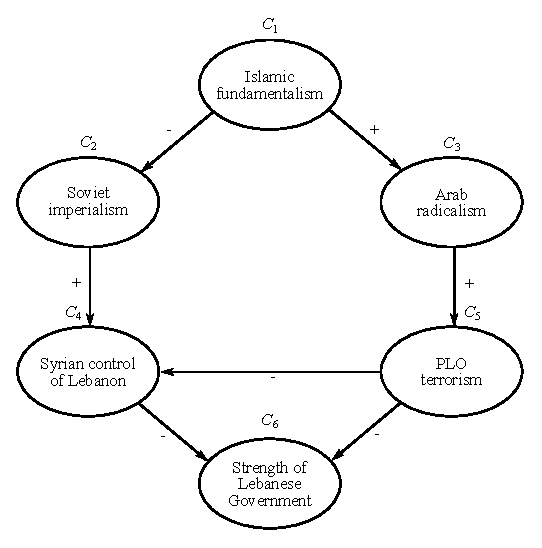
\includegraphics[scale=1]{kissinger}
    \caption{The Cognitive Map drawn by Kosko based on Kissinger's essay.}
  \end{center}
  \label{fig:kissingerCM}
\end{figure}

\begin{figure}[hbt]
  \sidecaption
  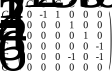
\includegraphics[scale=1.25]{kissingerMtx}
  \caption{The adjacency matrix of the CM based on Kissinger's essay.}
  \label{fig:kissingerMtx}
\end{figure}

It became quickly evident that the structure of a Cognitive Map imply too much limitations. The degree of causality, the levels of the causal effects (sometimes--often, little--much, etc.) cannot be expressed with the existing tool, and needs further development. Kosko introduced the Fuzzy Cognitive Map (FCM) \cite{b.kosko1986}, where the edges may have several causality values. This way the original CM turned into a bipolar fuzzy graph \cite{zhang1998yin}. Kosko also developed a fuzzy causal algebra for propagating causality in it, making the static analysis of the model possible. The concepts may affect other concepts indirectly because of the cyclic and non-feedforward structure of FCM.

\section{Simulations}
\label{sec:2}

The visual representation and formal description of models may help experts to review the structure of the studied system, but the real benefit of FCMs is the possibility of running simulations. This can be done by dynamic analysis \cite{kosko1988hidden}. Using a simple inference technique, the next state of concepts (also called the \emph{activation values} of concepts, based on the similarity of FCMs and artificial neural networks) can be calculated using their current state and the weight of connections among them \cite{dickerson1994virtual,tsadiras2008comparing}. This way what-if analysis can be performed which is very useful for decision makers.

\subsection{Inference rules}

Kosko defined the first, and still widely applied inference rule (Eq.~\ref{eq:Type1Inference}). In this case concepts are not allowed to directly influence themselves. With other words, a concept does not have ``memory'', technically speaking the edges must connect different concepts (i.e. self-loops are forbidden), but indirect feedbacks are still possible. Accordingly, the main diagonal of the connection matrix contains only zeros. These models are called FCMs of Type I \cite{stylios1999mathematical}.

\begin{equation}
\label{eq:Type1Inference}
A_{i}^{t+1} = f \left( \sum_{\substack{j=1\\j \ne i}}^{n} w_{ji}A_{j}^{t} \right)
\end{equation}

Here, $A_i^{t+1}$ is the activation value of concept $i$ at time step $t+1$, $n$ is the number of concepts and $f(\cdot)$ is the \emph{threshold} (transformation, squeezing) function. Without this function, the activation values of concepts may exceed or fall below their allowed extreme values.

FCMs of Type III allow concepts to take into account their current states during the calculation of the next state, and apply the inference rule defined by Eq.~\ref{eq:Type3Inference}. In this case, the main diagonal of the connection matrix may contain nonzero values, which are often ones in practice.

\begin{equation}
\label{eq:Type3Inference}
A_{i}^{t+1} = f \left( w_{ii}A_i^t + \sum_{\substack{j=1\\j \ne i}}^{n} w_{ji}A_{j}^{t} \right)
\end{equation}

FCMs of Type II also have a one step memory, but the weight of self-loops ($k_1$) are the same for all concepts. Moreover, the influence coming from other concepts can be limited as well ($k_2$, see Eqs.~\ref{eq:Type2Inference}, \ref{eq:Type2k}). 

\begin{equation}
\label{eq:Type2Inference}
A_{i}^{t+1} = f \left( k_1 A_i^t + k_2 \sum_{\substack{j=1\\j \ne i}}^{n} w_{ji}A_{j}^{t} \right)
\end{equation}

\begin{equation}
\label{eq:Type2k}
0 < k_1, k_2 \leq 1
\end{equation}

Papageorgiu suggested the re-scale inference rule (Eq.~\ref{eq:rescaleInference}) in \cite{papageorgioue.i.2011}, because problems emerged in cases where the initial values of concepts were 0 or 0.5, assuming that the initial states are known at all. This modified inference rule yielded more reliable and natural results than other FCM versions.

\begin{equation}
\label{eq:rescaleInference}
A_{i}^{t+1} = f \left( (2A_i^t-1) + \sum_{\substack{j=1\\j \ne i}}^{n} w_{ji}\cdot(2A_j^t-1) \right)
\end{equation}

\subsection{Threshold functions}

In general, the activation values are in the $A_{i}\in[0, 1]$ interval. Several threshold functions were published during the years, but the most widely applied one is the \emph{sigmoid} (\emph{logistics}) function (Eq.~\ref{eq:sigmoid}):

\begin{equation}
\label{eq:sigmoid}
f_{\textrm{sigmoid}}(x) = \frac{1}{1+e^{-\lambda x}}
\end{equation}

where the $\lambda > 0$ specifies the steepness of the function. It's typical value is 5. With greater values it approximates a binary function, with lower values a linear function (see Fig.~\ref{fig:lambdaSigmoid}). 

\begin{backgroundinformation}{Choosing an appropriate $\lambda$ value}
Is there an ``appropriate'' value of this parameter? According to Bueno and Salmeron \cite{buenoActivation}, the appropriate value should be found during an experimentation phase. As it was pointed out in \cite{hatwagnerm.f.koczyl.t.2015,parameterDependence}, the congergence speed and the final, stable values of concepts are heavily affected by the value of parameter $\lambda$ (see Fig.~\ref{fig:lambdaDependence}). Despite of the different results, different $\lambda$ values does not change the result of a simulation qualitatively, because the sigmoid function is strictly monotonically increasing. In practice, it is still worth to find an ``optimal'' value for $\lambda$, because sometimes the otherwise hardly different concept states may become distinguishable, and the order of concepts can be defined, if it is required. A possible method for ``lambda optimization'' is to maximize the standard deviation of final concept values (Fig.~\ref{fig:standardDeviation}) even by a quick local search algorithm, eg. the Golden Section Search.

\begin{figure}[hbt]
  \begin{center}
    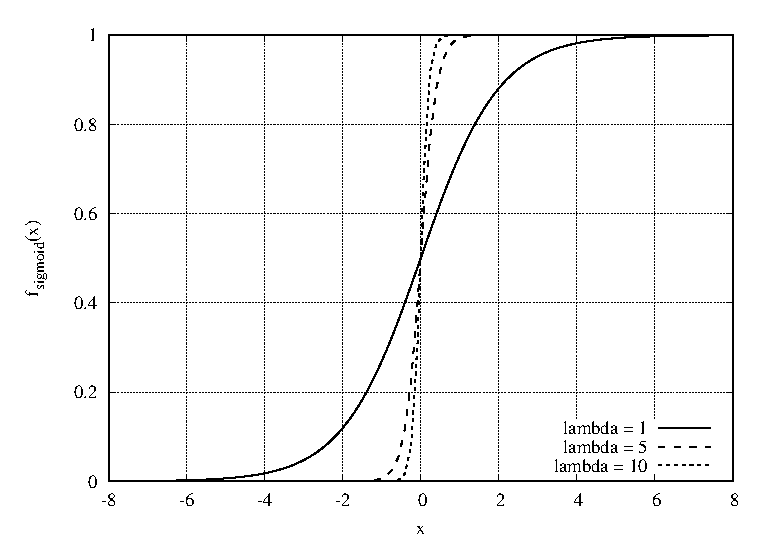
\includegraphics[scale=.8]{lambdaSigmoid.eps}
  \end{center}
  \caption{Steepness of the sigmoid function with various $\lambda$ parameters.}
  \label{fig:lambdaSigmoid}
\end{figure}

\begin{figure}[hbt]
  \begin{center}
    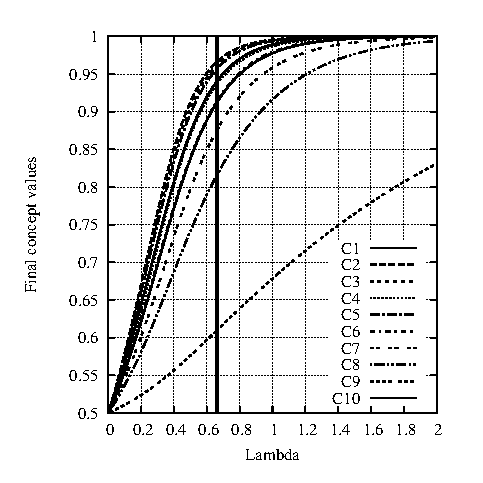
\includegraphics[scale=.9]{ascc2015plots/lambda.eps}
  \end{center}
  \caption{The final concept values of a Stakeholder Relationship Management System as function of parameter $\lambda$. $\lambda = 0.664$ maximized the standard deviation of concept values (marked with the thick vertical line).}
  \label{fig:lambdaDependence}
\end{figure}

\begin{figure}[hbt]
  \begin{center}
    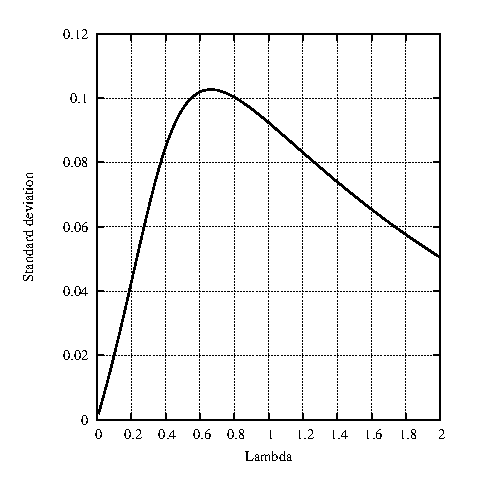
\includegraphics[scale=.9]{ascc2015plots/stdDev.eps}
  \end{center}
  \caption{Standard deviation of final concept values of a Stakeholder Relationship Management System calculated with different $\lambda$ values.}
  \label{fig:standardDeviation}
\end{figure}

Even if the value of $\lambda$ can be considered ``optimal'', a scalar value is unable to unleash the full modeling potencial of an FCM. In an extreme case, every concept may have its own, specific $\lambda$ value, in order to get more realistic predictions. This way, the inference rule defined by Eq.~\ref{eq:Type1Inference} can be re-written to Eq.~\ref{eq:inferenceMultilambda}, where $f_i$ represents the threshold function of concept $C_i$ that uses $\lambda_i$. This approach increases the number of model parameters, however. One of the benefits of using FCM was its simple structure, which can be understood easily by stakeholders, experts of different fields, and the values (initial states of concepts, connection weights) can be matched to real values or effects in a straightforward way. The values of $\lambda$ do not have trivial connection with any real world objects, however, and their values can be set with trial and error technique or computationally. It also increases the required computational power of applications because it increases the number of model parameters. A good balance can be found if some concepts have their own parameters, the others share a common value.

\begin{equation}
\label{eq:inferenceMultilambda}
A_{i}^{t+1} = f_i \left( \sum_{j=1}^{n} w_{ji}A_{j}^{t} \right)
\end{equation}

Concepts may be classified in three groups: if a concept influences the state of other concepts, but not affected by other concepts, it can be called an \emph{input} concept. Depending on the applied inference method, these concepts keep their initial values or their values can be sustained artificially (like ``sustained inputs'' in \cite{dickerson1994virtual}), therefore they do not need threshold function and parameter $\lambda$ neither. Another group of concepts is affected by other concepts but its elements do not influence the state of other concepts. In many applications, only these concepts are used for decision making, and they are called \emph{output} concepts. The remaining concepts are both affected by and they also affect other concepts, and are called \emph{intermediate} concepts \cite{boutalis2014system}.

If all output concepts have specific $\lambda$ values, and intermediate concepts have a common $\lambda$, the complexity of the model remains moderate but its forecasting ability can be increased as it happened in \cite{hatwagner2018two}. If historical time series data are available, $\lambda$s can be optimized with eg. the Big Bang -- Big Crunch algorithm \cite{yesilenginurbasleon2010}.
\end{backgroundinformation}

The \emph{sign} function (Eq.~\ref{eq:sign}) is also a popular threshold function, but because of the two available values, a concept can only be activated (1) or deactivated (0). 

\begin{equation}
\label{eq:sign}
f_{\textrm{sign}}(x) = \left\{
\begin{array}{ll}
1, & x>0, \\
0, & x \leq 0 \\
\end{array}
\right.
\end{equation}

In some cases the system to be modeled requires the activation values to be in $A_i\in [-1, +1]$, and different threshold functions have to be applied. If continuous states are allowed, the \emph{hyperbolic tangent} function (Eq.~\ref{eq:hyperbolicTangent}) is a possible choice:

\begin{equation}
\label{eq:hyperbolicTangent}
f_{\textrm{ht}}(x) = tanh(\lambda x) = \frac{e^{\lambda x}-e^{-\lambda x}}{e^{\lambda x}+e^{-\lambda x}}
\end{equation}

The $\lambda$ parameter can be used here as well, and has similar effect on the steepness of the function than on sigmoid function's (Fig.~\ref{fig:lambdaHT}).

\begin{figure}[hbt]
  \begin{center}
    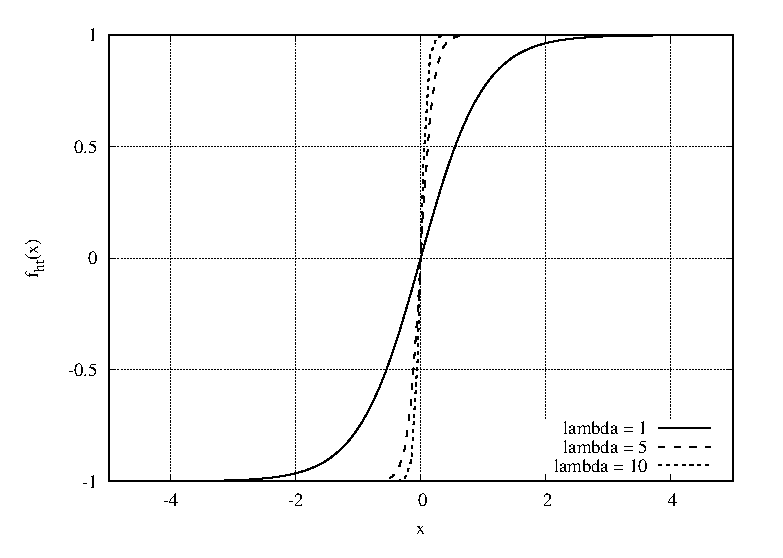
\includegraphics[scale=.8]{lambdaHT.eps}
  \end{center}
  \caption{Steepness of the hyperbolic tangent function with various $\lambda$ parameters.}
  \label{fig:lambdaHT}
\end{figure}

If only discrete states have to used, the \emph{trivalent} function (Eq.~\ref{eq:trivalent1}) can be the solution. The value 1 expresses the increasing, the value $-1$ expresses the decreasing and 0 means the stable state of a concept. A slightly modified version of this function can be found in \cite{yesil2014fcm} (Eq.~\ref{eq:trivalent2}).

\begin{equation}
\label{eq:trivalent1}
f_{\textrm{trivalent1}}(x) = \left\{
\begin{array}{ll}
1, & x>0, \\
0, & x=0, \\
-1,& x<0. \\
\end{array}
\right.
\end{equation}

\begin{equation}
\label{eq:trivalent2}
f_{\textrm{trivalent2}}(x) = \left\{
\begin{array}{ll}
1, & x \geq 0.5, \\
0, & -0.5 < x < 0.5, \\
-1,& x \leq -0.5. \\
\end{array}
\right.
\end{equation}

\subsection{Simulation outcomes}

During simulations, the states of concepts continuously evolve, until one of the three possible outcomes happens \cite{tsadiras2008comparing}:

\begin{enumerate}
  \item In most cases, the activation values converge very quickly to a stable state (equilibrium point, see Eq.~\ref{eq:fixedPoint}). These states are also called \emph{fixed points} (FPs). Depending on the connection matrix, initial state, inference rule, threshold function and its $\lambda$ parameter (if applied), a model may have multiple FPs.
  
  \begin{equation}
  \label{eq:fixedPoint}
  \exists t_{\textbf{FP}} \in \mathbb{N} : A_i^{t+1} = A_i^t, \forall t \geq t_{\textbf{FP}}, i=1, \dots, n
  \end{equation}
  
  \item Sometimes the system enters a \emph{limit cycle} (LC). In these cases after several time steps, a $T$ steps long sequence of state vectors starts to repeat (see Eq.~\ref{eq:limitCycle}).
  
  \begin{equation}
  \label{eq:limitCycle}
  \exists t_{\textbf{LC}}, T \in \mathbb{N} : A_i^{t+T} = A_i^t, \forall t \geq t_{\textbf{LC}}, i=1, \dots, n
  \end{equation}
  
  \item The system never stabilizes, behaves chaotically.
\end{enumerate}

It's easy to prove that bivalent and trivalent systems cannot behave chaotically. The process of simulations are deterministic, and the number of different state vectors is $2^n$ or $3^n$, respectively, where $n$ is the number of concepts. According to this, if the system is unstable, its states are going to repeat after $2^n$ or $3^n$ time steps, or earlier. FPs and LCs are related to the hidden patterns described in Kosko's work \cite{kosko1988hidden}.

In contrast, continuous state FCMs may enter practically infinite different states, thus chaotic behavior is possible. It happens especially often in case of Type III FCMs, which enter LCs frequently as well \cite{martchenko2003investigating}. Martchenko et al. also defined the condition of stability, too, which depends on the connection matrix.

Harmati et al. went further \cite{harmati2018existenceFCM} and determined the conditions of convergence and the number of FPs. According to their results, if the FCM uses sigmoid threshold function and the inequality

\begin{equation}
\label{eq:oneFPsigmoid}
||W||_F < \frac{4}{\lambda}
\end{equation}

holds, then the FCM has exactly one FP, without any LCs or chaotic patterns. Here $W$ is the connection matrix, $||\cdot||_F$ is the Frobenius-norm of the matrix defined by Eq.~\ref{eq:Frobenius}, and $\lambda$ is the steepness of the threshold function.

\begin{equation}
\label{eq:Frobenius}
||W||_F = \left( \sum_i \sum_j w_{ij}^2 \right)^{1/2}
\end{equation}

Similarly, if the hyperbolic tangent function is applied and Eq.~\ref{eq:oneFPhypTan} holds, the FCM has one and only one FP. These theorems are valid even if the connection matrix contains direct feedbacks.

\begin{equation}
\label{eq:oneFPhypTan}
||W||_F < \frac{1}{\lambda}
\end{equation}

Moreover, if the sigmoid or hyperbolic tangent threshold functions are used, and $W$ contains only non-negative elements than the FCM has FP, regardless of the value of $\lambda$. Similar contexts were also explored in case of some extended versions of FCM, the Grey FCMs \cite{harmati2018convergenceGFCM} and Fuzzy Set Valued Sigmoid FCMs \cite{harmati2018existenceFSVFCM}.

These are remarkable achievements because some of the behavioral properties of an FCM can be revealed without executing an exhaustive set of simulations, which is computationally very intensive. Unfortunately it is often unavoidable. If the model is made by experts, it may contain many subjective elements, eg. it is really hard to define the exact weight of a relationship. Even a small difference in the weights may lead to different behaviour, however. It is worth investigate the effect of small model modifications on behavioural properties, but it means a huge job which must be automated like in \cite{hatwagner2019banking,hatwagner2018improved}. The search space is huge for an exhaustive search hence Bacterial Evolutionary Algorithm \cite{nawa1998bacterial} was applied to generate and analyse the behavioral difference caused by slightly modified model versions and $\lambda$ values. If modified models with significantly different dynamic behaviour are found, experts are suggested to consider some changes on the model.

In most decision making tasks, stable states are the desired results. In these cases the future state of a system can be determined, and if that equilibrium state is undesirable, measures can be taken. There are some situations however, eg. time series predictions \cite{homenda2014modeling,homenda2017clustering,lu2014modeling}, when LCs or chaotic behavior seems very useful. Often extended versions of the original FCM are suggested to get better predictions.

\subsection{An example simulation}

Finally, an example FCM is given for illustration. The model has 5 concepts, their allowed values are in the interval [0,~1]. Kosko's original inference rule is applied (Eq.~\ref{eq:Type1Inference}), the threshold function is the sigmoid type (Eq.~\ref{eq:sigmoid}) with parameter $\lambda = 5$.

Formally, this model can be defined by a 4-tuple $(C, W, A, f)$, where $C = C_1, C_2,\dots, C_n$ is the set of $n=5$ concepts, function $W : (C_i,~C_j) \to w_{ij}$ associates the causal value $w_{ij} \in [-1,~+1]$ to each pair of concepts $(C_i,~C_j)$. These weights of directed edges are collected in the connection matrix denoted by $W_{nxn}$. Another function, $A : (C_i) \to A_i$ associates the activation value $A_i \in \mathbb{R}$ to each node $C_i$ at each time step $t = 1, 2,\dots, m$. The (sigmoid) threshold function $f : \mathbb{R} \to [0,~1]$ forces the activation values in their allowed range.

These are very general settings, and according to this, the dynamic behavior of the model is also very typical: the concepts' values converge after some time steps to their final values, to an equilibrium point.

\begin{table}[!t]
\caption{Connection matrix of the example FCM.}
\label{tab:exampleConnMtx}
\begin{tabular}{p{1cm}|p{1cm}p{1cm}p{1cm}p{1cm}p{1cm}}
\hline\noalign{\smallskip}
 & $C_1$ & $C_2$ & $C_3$ & $C_4$ & $C_5$ \\
\noalign{\smallskip}\svhline\noalign{\smallskip}
$C_1$ & 0 & 0.5 & 0.3 & 0 & 0 \\
$C_2$ & 0 & 0 & 0 & $-0.1$ & 0.35 \\
$C_3$ & 0 & $-0.1$ & 0 & $-0.2$ & 0.4 \\
$C_4$ & 0.4 & 0 & 0 & 0 & 0 \\
$C_5$ & $-0.7$ & 0 & 0 & 0 & 0 \\
\noalign{\smallskip}\hline\noalign{\smallskip}
\end{tabular}
\end{table}

\begin{table}[!t]
\caption{State vectors of the example FCM.}
\label{tab:exampleStates}
\begin{tabular}{p{1cm}p{1cm}p{1cm}p{1cm}p{1cm}p{1cm}}
\hline\noalign{\smallskip}
Time & $C_1$ & $C_2$ & $C_3$ & $C_4$ & $C_5$ \\
\noalign{\smallskip}\svhline\noalign{\smallskip}
$t_0$ & 0.00 & 0.50 & 1.00 & 0.50 & 0.00 \\
$t_1$ & 0.94 & 0.44 & 0.32 & 0.50 & 0.50 \\
$t_2$ & 0.83 & 0.65 & 0.57 & 0.87 & 0.04 \\
$t_3$ & 0.92 & 0.41 & 0.25 & 0.84 & 0.05 \\
$t_4$ & 0.80 & 0.42 & 0.28 & 0.86 & 0.04 \\
$t_5$ & 0.81 & 0.41 & 0.27 & 0.83 & 0.06 \\
$t_6$ & 0.81 & 0.42 & 0.28 & 0.84 & 0.05 \\
$t_7$ & 0.81 & 0.42 & 0.28 & 0.83 & 0.06 \\
$t_8$ & 0.81 & 0.42 & 0.28 & 0.84 & 0.05 \\
$t_9$ & 0.81 & 0.42 & 0.28 & 0.84 & 0.05 \\
\noalign{\smallskip}\hline\noalign{\smallskip}
\end{tabular}
\end{table}

\begin{figure}[hbt]
  \sidecaption
  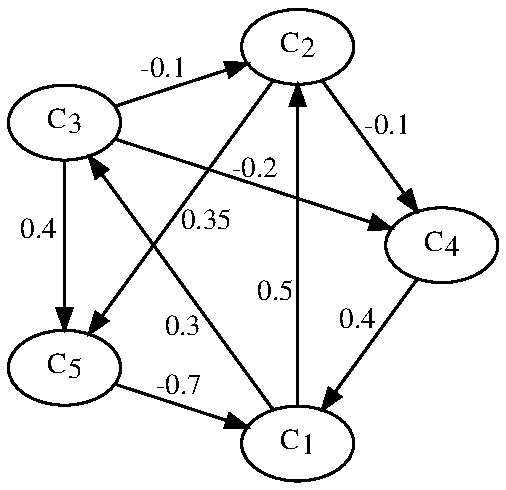
\includegraphics[scale=0.5]{simulation/graph.pdf}
  \caption{Graphical representation of the example FCM.}
  \label{fig:exampleGraph}
\end{figure}

\begin{figure}[hbt]
  \sidecaption
  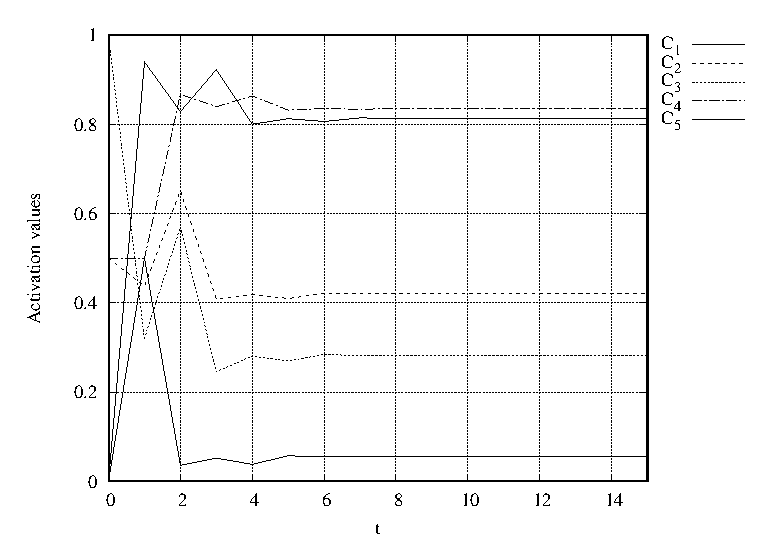
\includegraphics[scale=0.55]{simulation/simulation.eps}
  \caption{Convergence of concept activations during simulation.}
  \label{fig:exampleConvergence}
\end{figure}

\section{Creating a Fuzzy Cognitive Map model}

% \cite{kosko1988hidden} --> Szakértők, minél több, annál jobb, credibility weight, differential Hebbian learning
% \cite{papageorgiou2012learning} --> csak a gépi tanulási algoritmusokkal foglalkozik, jó összefoglaló

% fcm modellalkotás, tanulás, modellredukció

%however, for multiline equations we recommend to use the \verb|eqnarray| environment\footnote{In physics texts please activate the class option \texttt{vecphys} to depict your vectors in \textbf{\itshape boldface-italic} type - as is customary for a wide range of physical subjects}.
%\begin{eqnarray}
%\left|\nabla U_{\alpha}^{\mu}(y)\right| &\le&\frac1{d-\alpha}\int
%\left|\nabla\frac1{|\xi-y|^{d-\alpha}}\right|\,d\mu(\xi) =
%\int \frac1{|\xi-y|^{d-\alpha+1}} \,d\mu(\xi)  \\
%&=&(d-\alpha+1) \int\limits_{d(y)}^\infty
%\frac{\mu(B(y,r))}{r^{d-\alpha+2}}\,dr \le (d-\alpha+1)
%\int\limits_{d(y)}^\infty \frac{r^{d-\alpha}}{r^{d-\alpha+2}}\,dr
%\label{eq:01}
%\end{eqnarray}

\subsection{Subsection Heading}
\label{subsec:2}
Instead of simply listing headings of different levels we recommend to let every heading be followed by at least a short passage of text.  Further on please use the \LaTeX\ automatism for all your cross-references\index{cross-references} and citations\index{citations} as has already been described in Sect.~\ref{sec:2}.

\begin{quotation}
Please do not use quotation marks when quoting texts! Simply use the \verb|quotation| environment -- it will automatically be rendered in line with the preferred layout.
\end{quotation}


\subsubsection{Subsubsection Heading}
Instead of simply listing headings of different levels we recommend to let every heading be followed by at least a short passage of text.  Further on please use the \LaTeX\ automatism for all your cross-references and citations as has already been described in Sect.~\ref{subsec:2}, see also Fig.~\ref{fig:1}\footnote{If you copy text passages, figures, or tables from other works, you must obtain \textit{permission} from the copyright holder (usually the original publisher). Please enclose the signed permission with the manuscript. The sources\index{permission to print} must be acknowledged either in the captions, as footnotes or in a separate section of the book.}

Please note that the first line of text that follows a heading is not indented, whereas the first lines of all subsequent paragraphs are.

% For figures use
%
\begin{figure}[b]
\sidecaption
% Use the relevant command for your figure-insertion program
% to insert the figure file.
% For example, with the graphicx style use
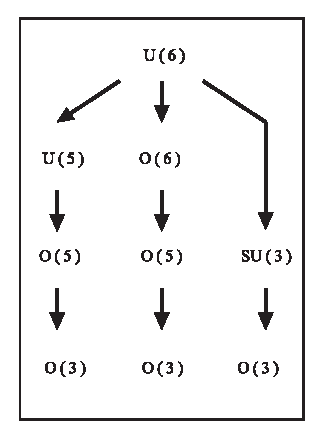
\includegraphics[scale=.65]{figure}
%
% If no graphics program available, insert a blank space i.e. use
%\picplace{5cm}{2cm} % Give the correct figure height and width in cm
%
\caption{If the width of the figure is less than 7.8 cm use the \texttt{sidecapion} command to flush the caption on the left side of the page. If the figure is positioned at the top of the page, align the sidecaption with the top of the figure -- to achieve this you simply need to use the optional argument \texttt{[t]} with the \texttt{sidecaption} command}
\label{fig:1}       % Give a unique label
\end{figure}


\paragraph{Paragraph Heading} %
Instead of simply listing headings of different levels we recommend to let every heading be followed by at least a short passage of text.  Further on please use the \LaTeX\ automatism for all your cross-references and citations as has already been described in Sect.~\ref{sec:2}.

Please note that the first line of text that follows a heading is not indented, whereas the first lines of all subsequent paragraphs are.

For typesetting numbered lists we recommend to use the \verb|enumerate| environment -- it will automatically rendered in line with the preferred layout.

\begin{enumerate}
\item{Livelihood and survival mobility are oftentimes coutcomes of uneven socioeconomic development.}
\begin{enumerate}
\item{Livelihood and survival mobility are oftentimes coutcomes of uneven socioeconomic development.}
\item{Livelihood and survival mobility are oftentimes coutcomes of uneven socioeconomic development.}
\end{enumerate}
\item{Livelihood and survival mobility are oftentimes coutcomes of uneven socioeconomic development.}
\end{enumerate}


\subparagraph{Subparagraph Heading} In order to avoid simply listing headings of different levels we recommend to let every heading be followed by at least a short passage of text. Use the \LaTeX\ automatism for all your cross-references and citations as has already been described in Sect.~\ref{sec:2}, see also Fig.~\ref{fig:2}.

For unnumbered list we recommend to use the \verb|itemize| environment -- it will automatically be rendered in line with the preferred layout.

\begin{itemize}
\item{Livelihood and survival mobility are oftentimes coutcomes of uneven socioeconomic development, cf. Table~\ref{tab:1}.}
\begin{itemize}
\item{Livelihood and survival mobility are oftentimes coutcomes of uneven socioeconomic development.}
\item{Livelihood and survival mobility are oftentimes coutcomes of uneven socioeconomic development.}
\end{itemize}
\item{Livelihood and survival mobility are oftentimes coutcomes of uneven socioeconomic development.}
\end{itemize}

\begin{figure}[t]
\sidecaption[t]
% Use the relevant command for your figure-insertion program
% to insert the figure file.
% For example, with the option graphics use
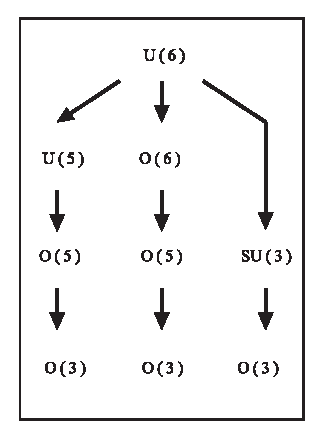
\includegraphics[scale=.65]{figure}
%
% If no graphics program available, insert a blank space i.e. use
%\picplace{5cm}{2cm} % Give the correct figure height and width in cm
%
%\caption{Please write your figure caption here}
\caption{If the width of the figure is less than 7.8 cm use the \texttt{sidecapion} command to flush the caption on the left side of the page. If the figure is positioned at the top of the page, align the sidecaption with the top of the figure -- to achieve this you simply need to use the optional argument \texttt{[t]} with the \texttt{sidecaption} command}
\label{fig:2}       % Give a unique label
\end{figure}

\runinhead{Run-in Heading Boldface Version} Use the \LaTeX\ automatism for all your cross-references and citations as has already been described in Sect.~\ref{sec:2}.

\subruninhead{Run-in Heading Boldface and Italic Version} Use the \LaTeX\ automatism for all your cross-refer\-ences and citations as has already been described in Sect.~\ref{sec:2}\index{paragraph}.

\subsubruninhead{Run-in Heading Displayed Version} Use the \LaTeX\ automatism for all your cross-refer\-ences and citations as has already been described in Sect.~\ref{sec:2}\index{paragraph}.
% Use the \index{} command to code your index words
%
% For tables use
%
\begin{table}[!t]
\caption{Please write your table caption here}
\label{tab:1}       % Give a unique label
%
% Follow this input for your own table layout
%
\begin{tabular}{p{2cm}p{2.4cm}p{2cm}p{4.9cm}}
\hline\noalign{\smallskip}
Classes & Subclass & Length & Action Mechanism  \\
\noalign{\smallskip}\svhline\noalign{\smallskip}
Translation & mRNA$^a$  & 22 (19--25) & Translation repression, mRNA cleavage\\
Translation & mRNA cleavage & 21 & mRNA cleavage\\
Translation & mRNA  & 21--22 & mRNA cleavage\\
Translation & mRNA  & 24--26 & Histone and DNA Modification\\
\noalign{\smallskip}\hline\noalign{\smallskip}
\end{tabular}
$^a$ Table foot note (with superscript)
\end{table}
%
\section{Section Heading}
\label{sec:3}
% Always give a unique label
% and use \ref{<label>} for cross-references
% and \cite{<label>} for bibliographic references
% use \sectionmark{}
% to alter or adjust the section heading in the running head
Instead of simply listing headings of different levels we recommend to let every heading be followed by at least a short passage of text.  Further on please use the \LaTeX\ automatism for all your cross-references and citations as has already been described in Sect.~\ref{sec:2}.

Please note that the first line of text that follows a heading is not indented, whereas the first lines of all subsequent paragraphs are.

If you want to list definitions or the like we recommend to use the enhanced \verb|description| environment -- it will automatically rendered in line with the preferred layout.

\begin{description}[Type 1]
\item[Type 1]{That addresses central themes pertainng to migration, health, and disease. In Sect.~\ref{sec:1}, Wilson discusses the role of human migration in infectious disease distributions and patterns.}
\item[Type 2]{That addresses central themes pertainng to migration, health, and disease. In Sect.~\ref{subsec:2}, Wilson discusses the role of human migration in infectious disease distributions and patterns.}
\end{description}

\subsection{Subsection Heading} %
In order to avoid simply listing headings of different levels we recommend to let every heading be followed by at least a short passage of text. Use the \LaTeX\ automatism for all your cross-references and citations citations as has already been described in Sect.~\ref{sec:2}.

Please note that the first line of text that follows a heading is not indented, whereas the first lines of all subsequent paragraphs are.

\begin{svgraybox}
If you want to emphasize complete paragraphs of texts we recommend to use the newly defined class option \verb|graybox| and the newly defined environment \verb|svgraybox|. This will produce a 15 percent screened box 'behind' your text.

If you want to emphasize complete paragraphs of texts we recommend to use the newly defined class option and environment \verb|svgraybox|. This will produce a 15 percent screened box 'behind' your text.
\end{svgraybox}


\subsubsection{Subsubsection Heading}
Instead of simply listing headings of different levels we recommend to let every heading be followed by at least a short passage of text.  Further on please use the \LaTeX\ automatism for all your cross-references and citations as has already been described in Sect.~\ref{sec:2}.

Please note that the first line of text that follows a heading is not indented, whereas the first lines of all subsequent paragraphs are.

\begin{theorem}
Theorem text goes here.
\end{theorem}
%
% or
%
\begin{definition}
Definition text goes here.
\end{definition}

\begin{proof}
%\smartqed
Proof text goes here.
%\qed
\end{proof}

\paragraph{Paragraph Heading} %
Instead of simply listing headings of different levels we recommend to let every heading be followed by at least a short passage of text.  Further on please use the \LaTeX\ automatism for all your cross-references and citations as has already been described in Sect.~\ref{sec:2}.

Note that the first line of text that follows a heading is not indented, whereas the first lines of all subsequent paragraphs are.
%
% For built-in environments use
%
\begin{theorem}
Theorem text goes here.
\end{theorem}
%
\begin{definition}
Definition text goes here.
\end{definition}
%
\begin{proof}
%\smartqed
Proof text goes here.
%\qed
\end{proof}
%
\begin{trailer}{Trailer Head}
If you want to emphasize complete paragraphs of texts in an \verb|Trailer Head| we recommend to
use  \begin{verbatim}\begin{trailer}{Trailer Head}
...
\end{trailer}\end{verbatim}
\end{trailer}
%
\begin{question}{Questions}
If you want to emphasize complete paragraphs of texts in an \verb|Questions| we recommend to
use  \begin{verbatim}\begin{question}{Questions}
...
\end{question}\end{verbatim}
\end{question}
\eject%
\begin{important}{Important}
If you want to emphasize complete paragraphs of texts in an \verb|Important| we recommend to
use  \begin{verbatim}\begin{important}{Important}
...
\end{important}\end{verbatim}
\end{important}
%
\begin{warning}{Attention}
If you want to emphasize complete paragraphs of texts in an \verb|Attention| we recommend to
use  \begin{verbatim}\begin{warning}{Attention}
...
\end{warning}\end{verbatim}
\end{warning}

\begin{programcode}{Program Code}
If you want to emphasize complete paragraphs of texts in an \verb|Program Code| we recommend to
use

\verb|\begin{programcode}{Program Code}|

\verb|\begin{verbatim}...\end{verbatim}|

\verb|\end{programcode}|

\end{programcode}
%
\begin{tips}{Tips}
If you want to emphasize complete paragraphs of texts in an \verb|Tips| we recommend to
use  \begin{verbatim}\begin{tips}{Tips}
...
\end{tips}\end{verbatim}
\end{tips}
\eject
%
\begin{overview}{Overview}
If you want to emphasize complete paragraphs of texts in an \verb|Overview| we recommend to
use  \begin{verbatim}\begin{overview}{Overview}
...
\end{overview}\end{verbatim}
\end{overview}
\begin{backgroundinformation}{Background Information}
If you want to emphasize complete paragraphs of texts in an \verb|Background|
\verb|Information| we recommend to
use

\verb|\begin{backgroundinformation}{Background Information}|

\verb|...|

\verb|\end{backgroundinformation}|
\end{backgroundinformation}
\begin{legaltext}{Legal Text}
If you want to emphasize complete paragraphs of texts in an \verb|Legal Text| we recommend to
use  \begin{verbatim}\begin{legaltext}{Legal Text}
...
\end{legaltext}\end{verbatim}
\end{legaltext}
%
\begin{acknowledgement}
If you want to include acknowledgments of assistance and the like at the end of an individual chapter please use the \verb|acknowledgement| environment -- it will automatically be rendered in line with the preferred layout.
\end{acknowledgement}
%
\section*{Appendix}
\addcontentsline{toc}{section}{Appendix}
%
%
When placed at the end of a chapter or contribution (as opposed to at the end of the book), the numbering of tables, figures, and equations in the appendix section continues on from that in the main text. Hence please \textit{do not} use the \verb|appendix| command when writing an appendix at the end of your chapter or contribution. If there is only one the appendix is designated ``Appendix'', or ``Appendix 1'', or ``Appendix 2'', etc. if there is more than one.

\begin{equation}
a \times b = c
\end{equation}

%%%%%%%%%%%%%%%%%%%%%%%% referenc.tex %%%%%%%%%%%%%%%%%%%%%%%%%%%%%%
% sample references
% %
% Use this file as a template for your own input.
%
%%%%%%%%%%%%%%%%%%%%%%%% Springer-Verlag %%%%%%%%%%%%%%%%%%%%%%%%%%
%
% BibTeX users please use
\bibliographystyle{plain}
\bibliography{../hfmbibfile}
%
%\biblstarthook{References may be \textit{cited} in the text either by number (preferred) or by author/year.\footnote{Make sure that all references from the list are cited in the text. Those not cited should be moved to a separate \textit{Further Reading} section or chapter.} If the citatiion in the text is numbered, the reference list should be arranged in ascending order. If the citation in the text is author/year, the reference list should be \textit{sorted} alphabetically and if there are several works by the same author, the following order should be used:
%\begin{enumerate}
%\item all works by the author alone, ordered chronologically by year of publication
%\item all works by the author with a coauthor, ordered alphabetically by coauthor
%\item all works by the author with several coauthors, ordered chronologically by year of publication.
%\end{enumerate}
%The \textit{styling} of references\footnote{Always use the standard abbreviation of a journal's name according to the ISSN \textit{List of Title Word Abbreviations}, see \url{http://www.issn.org/en/node/344}} depends on the subject of your book:
%\begin{itemize}
%\item The \textit{two} recommended styles for references in books on \textit{mathematical, physical, statistical and computer sciences} are depicted in ~\cite{science-contrib, science-online, science-mono, science-journal, science-DOI} and ~\cite{phys-online, phys-mono, phys-journal, phys-DOI, phys-contrib}.
%\item Examples of the most commonly used reference style in books on \textit{Psychology, Social Sciences} are~\cite{psysoc-mono, psysoc-online,psysoc-journal, psysoc-contrib, psysoc-DOI}.
%\item Examples for references in books on \textit{Humanities, Linguistics, Philosophy} are~\cite{humlinphil-journal, humlinphil-contrib, humlinphil-mono, humlinphil-online, humlinphil-DOI}.
%\item Examples of the basic Springer Nature style used in publications on a wide range of subjects such as \textit{Computer Science, Economics, Engineering, Geosciences, Life Sciences, Medicine, Biomedicine} are ~\cite{basic-contrib, basic-online, basic-journal, basic-DOI, basic-mono}. 
%\end{itemize}
%}

%\begin{thebibliography}{99.}%
%% and use \bibitem to create references.
%%
%% Use the following syntax and markup for your references if 
%% the subject of your book is from the field 
%% "Mathematics, Physics, Statistics, Computer Science"
%%
%% Contribution 
%\bibitem{science-contrib} Broy, M.: Software engineering --- from auxiliary to key technologies. In: Broy, M., Dener, E. (eds.) Software Pioneers, pp. 10-13. Springer, Heidelberg (2002)
%%
%% Online Document
%\bibitem{science-online} Dod, J.: Effective substances. In: The Dictionary of Substances and Their Effects. Royal Society of Chemistry (1999) Available via DIALOG. \\
%\url{http://www.rsc.org/dose/title of subordinate document. Cited 15 Jan 1999}
%%
%% Monograph
%\bibitem{science-mono} Geddes, K.O., Czapor, S.R., Labahn, G.: Algorithms for Computer Algebra. Kluwer, Boston (1992) 
%%
%% Journal article
%\bibitem{science-journal} Hamburger, C.: Quasimonotonicity, regularity and duality for nonlinear systems of partial differential equations. Ann. Mat. Pura. Appl. \textbf{169}, 321--354 (1995)
%%
%% Journal article by DOI
%\bibitem{science-DOI} Slifka, M.K., Whitton, J.L.: Clinical implications of dysregulated cytokine production. J. Mol. Med. (2000) doi: 10.1007/s001090000086 
%%
%\bigskip

%% Use the following (APS) syntax and markup for your references if 
%% the subject of your book is from the field 
%% "Mathematics, Physics, Statistics, Computer Science"
%%
%% Online Document
%\bibitem{phys-online} J. Dod, in \textit{The Dictionary of Substances and Their Effects}, Royal Society of Chemistry. (Available via DIALOG, 1999), 
%\url{http://www.rsc.org/dose/title of subordinate document. Cited 15 Jan 1999}
%%
%% Monograph
%\bibitem{phys-mono} H. Ibach, H. L\"uth, \textit{Solid-State Physics}, 2nd edn. (Springer, New York, 1996), pp. 45-56 
%%
%% Journal article
%\bibitem{phys-journal} S. Preuss, A. Demchuk Jr., M. Stuke, Appl. Phys. A \textbf{61}
%%
%% Journal article by DOI
%\bibitem{phys-DOI} M.K. Slifka, J.L. Whitton, J. Mol. Med., doi: 10.1007/s001090000086
%%
%% Contribution 
%\bibitem{phys-contrib} S.E. Smith, in \textit{Neuromuscular Junction}, ed. by E. Zaimis. Handbook of Experimental Pharmacology, vol 42 (Springer, Heidelberg, 1976), p. 593
%%
%\bigskip
%%
%% Use the following syntax and markup for your references if 
%% the subject of your book is from the field 
%% "Psychology, Social Sciences"
%%
%%
%% Monograph
%\bibitem{psysoc-mono} Calfee, R.~C., \& Valencia, R.~R. (1991). \textit{APA guide to preparing manuscripts for journal publication.} Washington, DC: American Psychological Association.
%%
%% Online Document
%\bibitem{psysoc-online} Dod, J. (1999). Effective substances. In: The dictionary of substances and their effects. Royal Society of Chemistry. Available via DIALOG. \\
%\url{http://www.rsc.org/dose/Effective substances.} Cited 15 Jan 1999.
%%
%% Journal article
%\bibitem{psysoc-journal} Harris, M., Karper, E., Stacks, G., Hoffman, D., DeNiro, R., Cruz, P., et al. (2001). Writing labs and the Hollywood connection. \textit{J Film} Writing, 44(3), 213--245.
%%
%% Contribution 
%\bibitem{psysoc-contrib} O'Neil, J.~M., \& Egan, J. (1992). Men's and women's gender role journeys: Metaphor for healing, transition, and transformation. In B.~R. Wainrig (Ed.), \textit{Gender issues across the life cycle} (pp. 107--123). New York: Springer.
%%
%% Journal article by DOI
%\bibitem{psysoc-DOI}Kreger, M., Brindis, C.D., Manuel, D.M., Sassoubre, L. (2007). Lessons learned in systems change initiatives: benchmarks and indicators. \textit{American Journal of Community Psychology}, doi: 10.1007/s10464-007-9108-14.
%%
%%
%% Use the following syntax and markup for your references if 
%% the subject of your book is from the field 
%% "Humanities, Linguistics, Philosophy"
%%
%\bigskip
%%
%% Journal article
%\bibitem{humlinphil-journal} Alber John, Daniel C. O'Connell, and Sabine Kowal. 2002. Personal perspective in TV interviews. \textit{Pragmatics} 12:257--271
%%
%% Contribution 
%\bibitem{humlinphil-contrib} Cameron, Deborah. 1997. Theoretical debates in feminist linguistics: Questions of sex and gender. In \textit{Gender and discourse}, ed. Ruth Wodak, 99--119. London: Sage Publications.
%%
%% Monograph
%\bibitem{humlinphil-mono} Cameron, Deborah. 1985. \textit{Feminism and linguistic theory.} New York: St. Martin's Press.
%%
%% Online Document
%\bibitem{humlinphil-online} Dod, Jake. 1999. Effective substances. In: The dictionary of substances and their effects. Royal Society of Chemistry. Available via DIALOG. \\
%http://www.rsc.org/dose/title of subordinate document. Cited 15 Jan 1999
%%
%% Journal article by DOI
%\bibitem{humlinphil-DOI} Suleiman, Camelia, Daniel C. O'Connell, and Sabine Kowal. 2002. `If you and I, if we, in this later day, lose that sacred fire...': Perspective in political interviews. \textit{Journal of Psycholinguistic Research}. doi: 10.1023/A:1015592129296.
%%
%%
%%
%\bigskip
%%
%%
%% Use the following syntax and markup for your references if 
%% the subject of your book is from the field 
%% "Computer Science, Economics, Engineering, Geosciences, Life Sciences"
%%
%%
%% Contribution 
%\bibitem{basic-contrib} Brown B, Aaron M (2001) The politics of nature. In: Smith J (ed) The rise of modern genomics, 3rd edn. Wiley, New York 
%%
%% Online Document
%\bibitem{basic-online} Dod J (1999) Effective Substances. In: The dictionary of substances and their effects. Royal Society of Chemistry. Available via DIALOG. \\
%\url{http://www.rsc.org/dose/title of subordinate document. Cited 15 Jan 1999}
%%
%% Journal article by DOI
%\bibitem{basic-DOI} Slifka MK, Whitton JL (2000) Clinical implications of dysregulated cytokine production. J Mol Med, doi: 10.1007/s001090000086
%%
%% Journal article
%\bibitem{basic-journal} Smith J, Jones M Jr, Houghton L et al (1999) Future of health insurance. N Engl J Med 965:325--329
%%
%% Monograph
%\bibitem{basic-mono} South J, Blass B (2001) The future of modern genomics. Blackwell, London 
%%
%\end{thebibliography}

\end{document}
